\section{Theorie}
\label{sec:Theorie}

\subsection{Erzeugung der Röntgenstrahlung und dessen Bremsspektrum}

Um Röntgenstrahlung zu erzeugen, wird in einer evakuierten Röhre eine Glühkatode erhitzt und die frei werdenden Elektronen beschleunigen hin zur Anode.
Je nach dem aus welchem Material die Anode besteht, entsteht die für das Material typische Röntgenstrahlung mit einem kontinuierlichen Bremsspektrum.
Die Bremsstrahlung entsteht, wenn ein Elektron in dem Coulombfeld eines Atoms abgebremst wird.
Dabei kann das Elektron einen Teil oder seine gesamte Energie in Form von Photonen abgeben. Deswegen ist das Bremsspektrum ein kontinuierliches Spektrum.
Die kleinste Wellenlänge wird dabei erreicht, wenn das Elektron seine gesamte Energie verliert.\\
Dies kann mit \autoref{eq:breakspec} berechnet werden. $U$ entspricht dabei der Beschleunigungsspannung und $e_0$ der Ladung des Elektrons.

\begin{equation}
    \lambda_{min} = \frac{h\cdot c}{e_0U}
    \label{eq:breakspec}
\end{equation}

Hierbei wird das Anodenmaterial ionisiert, was dazu führt, dass die atomgebundenen Elektronen die Schale wechseln können.

\subsection{Die Bragg'sche Bedingung}

Um das Röntgenlicht zu analysieren, wird die Bragg'sche Reflexion verwendet.\\
Hierbei werden die Photonen unter einem bestimmten Winkel $\alpha$ an einen Gitterkristall gesendet, sodass konstruktive Interferenz entsteht.
Zusammen mit der Gitterkonstante $d$ und der Beugungsordnung $n$, lässt sich damit die Wellenlänge nachweisen.
Die Formel der Bragg'schen Bedingung lautet:

\begin{equation}
    2d\sin{\alpha} = n\cdot \lambda
    \label{eq:bragg}
\end{equation}

\subsection{Charakteristische Linien und Absorption}

Die charakteristischen Röntgenlinien entstehen, wenn die atomgebundenen Elektronen die Schale wechseln.\\
Dabei hängen die entstehenden Wellenlängen vom Anodenmaterial ab.

\begin{figure}[htbp]
    \centering
    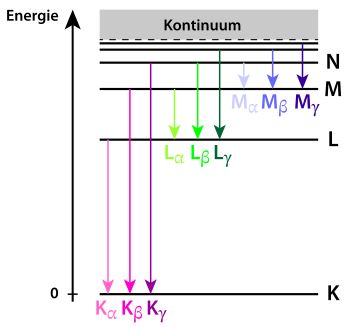
\includegraphics[scale=0.6]{content/992Charakteristische Röntgenstrahlung- Bezeichnungen der Übergänge.png}
    \caption{Veranschaulichung der Übergänge in der Elektronenhülle\cite{leifi}.}
    \label{fig:uebergang}
\end{figure}

In \autoref{fig:uebergang} sind die einzelnen Übergänge in den Schalen aufgetragen.
Dabei entspricht der K-Strich der Schale $n=1$ und der N-Strich $n=4$.
Beim Übergang eines Elektrons von einer höheren Schale zu einer niedrigeren, gibt es Energie ab.
Diese setzt sich aus der \textit{Rydbergenergie} $R_{\infty}$, einer effektiven Größe $z_{eff} = z\ -\ \sigma$ und den Schalen des Atoms zusammen:
\begin{equation}
    E_{m,n} = R_{\infty}z_{eff_{m,n}}^2\left(\frac{1}{n^2}\ -\ \frac{1}{m^2}\right)
    \label{eq:enrgy}
\end{equation}
$\sigma$ ist die Abschirmkonstante, die für jedes Elektron unterschiedlich ist.\\
Ein Elektron auf der n-ten Schale besitzt eine Bindungsenergie $E_n$:

\begin{equation}
    E_n = -R_{\infty}z_{eff}^2\cdot\frac{1}{n^2}
    \label{eq:bind}
\end{equation}

Wenn die Kernladungszahl $z$ zu groß ist, treten relativistische Effekte im Atom auf.
Das berücksichtigt die \textit{Sommerfeldsche Feinstrukturformel} in \autoref{eq:sommer}.

\begin{equation}
    E_{n,j} = -R_{\infty}\left(z_{eff,1}^2\cdot \frac{1}{n^2}\ +\ \alpha^2z_{eff,2}^4\cdot\frac{1}{n^3}\left(\frac{1}{j+\frac{1}{2}}\ -\ \frac{3}{4n}\right)\right)
    \label{eq:sommer}
\end{equation}

Hierbei ist $\alpha$ die Sommerfeldsche Feinstrukturkonstante und $j$ der Gesamtdrehimpuls des Elektrons.\\
Wird nur das Elektron aus der K-Kante betrachtet, also $n=1$, dann lässt sich $\sigma_K$ bestimmen aus:

\begin{equation}
    \sigma_K = Z\ -\ \sqrt{\frac{E_K}{R_{\infty}}\ -\ \frac{\alpha^2Z^4}{4}}
    \label{eq:sigma}
\end{equation}

Die Formeln für eine Abschätzung von $\sigma_{1,2,3}$ lauten:
\begin{align}
    \sigma_1 = Z\ -\ \sqrt{\frac{E_{abs}}{R_{\infty}}} \notag \\
    \sigma_2 = Z\ -\ \sqrt{4\left(Z\ -\ \sigma_1\right)^2\ -\ 4\cdot \frac{E_{K_{\alpha}}}{R_{\infty}}} \label{sigma1}\\
    \sigma_3 = Z\ -\ \sqrt{9\left(Z\ -\ \sigma_1\right)^2\ -\ 9\cdot \frac{E_{K_{\beta}}}{R_{\infty}}} \notag
\end{align}

Um das Auflösungsvermögen von charakteristischen Linien zu ermitteln benötigt man die Halbwertsbreite.\\
Die Halbwertsbreite gibt an, wie breit der Peak bei der Hälfte des Maximalwerts ist. 
Aus der Energiedifferenz der beiden Werte, die die Breite markieren, kann das Auflösungsvermögen errechnet werden:

\begin{equation}
    A = \frac{E_K}{\Delta E_{FWHM}}
    \label{eq:aufloes}
\end{equation}

Wenn die Röntgenstrahlung absorbiert wird, so nimmt der \textit{Absorptionskoeffizient} mit zunehmender Energie der Strahlung ab.
Übersteigt die Energie jedoch die Bindungenergie des Elektrons aus der nächsten inneren Schale, steigt der Absorptionskoeffizient rasch an.
Die Lage der Absorptionskanten lässt sich durch \autoref{eq:cunts} berechnen.

\begin{equation}
    h\ v_{abs} = E_n\ -\ E_{\infty}
    \label{eq:cunts}
\end{equation}

